% \documentclass[draft]{article}
\documentclass{article}

% % if you need to pass options to natbib, use, e.g.:
% \PassOptionsToPackage{round,sort&compress}{natbib}
% % before loading neurips_2019

% to compile a camera-ready version, add the [final] option, e.g.:
% \usepackage[nonatbib,final]{neurips_2019}
% to compile a preprint version, e.g., for submission to arXiv, add
% add the [preprint] option:
\usepackage[nonatbib,preprint]{neurips_2019}
% \usepackage[nonatbib]{neurips_2019}

% Bib config
\usepackage[
    backend=biber,
    style=authoryear,
    maxcitenames=2,
    maxbibnames=99,
    giveninits=true,
    uniquename=init,
    natbib=true,
    dashed=false
]{biblatex}

% \DeclareNameAlias{sortname}{last-first}
\DeclareNameAlias{sortname}{first-last}
\setlength\bibitemsep{0.45\baselineskip}

\AtEveryBibitem{%
    \clearfield{month}
    \clearfield{isbn}
    \clearfield{issn}
    % \clearfield{doi}
    \clearfield{pages}
    
    % \ifentrytype{online}{}{% Remove url except for @online
        % \clearfield{url}
    % }
}
\addbibresource{library.bib}

\usepackage[utf8]{inputenc} % allow utf-8 input
\usepackage[T1]{fontenc}    % use 8-bit T1 fonts
\usepackage{hyperref}       % hyperlinks
\usepackage{url}            % simple URL typesetting
\usepackage{booktabs}       % professional-quality tables
\usepackage{amsfonts}       % blackboard math symbols
\usepackage{amsmath}    % aligned etc
\usepackage{nicefrac}       % compact symbols for 1/2, etc.
\usepackage{microtype}      % microtypography
\usepackage{appendix}

\usepackage{mathtools} % for DeclarePairedDelimiter

\usepackage{floatrow}  % for MOHART
\usepackage{tabularx}  % for MOHART

\usepackage{amsthm}   % for tighter bounds
\usepackage{thmtools} 	% for tighter bounds
\usepackage{thm-restate}  % for tighter bounds
\usepackage{cancel}
\usepackage{wrapfig}

% for RRWS and TB
\usepackage{tikz}
\usetikzlibrary{calc,backgrounds,positioning,bayesnet,arrows.meta,patterns,fit,trees}


\usepackage[acronym,smallcaps,nowarn,section,nogroupskip,nonumberlist]{glossaries}

\usepackage{todonotes}
\usepackage[linesnumbered,ruled,vlined]{algorithm2e}
\usepackage{bm} % uniform bold

\usepackage{paralist}
\usepackage{enumitem} % nicer description

\usepackage{mlmacros} % nice macros for loss, kl, probabilities etc
\usepackage[nameinlink,capitalise]{cleveref} % better ref handling

\newcommand*{\defeq}{\mathrel{\vcenter{\baselineskip0.5ex \lineskiplimit0pt
                     \hbox{\scriptsize.}\hbox{\scriptsize.}}}%
                     =}

\presetkeys{todonotes}{%
  backgroundcolor=blue!10!white,
  linecolor=blue!10!white,
  bordercolor=blue!10!white
}{}


\usepackage[skip=5pt,font=small]{caption}
\usepackage{subcaption}

\usepackage{graphicx}
\graphicspath{{figures/}}
\usepackage[export]{adjustbox}

\usepackage{colortbl}  % for \rowcolor

% section spacing
\usepackage{titlesec}

%\titlespacing*{\section}{0pt}{.1\baselineskip}{.1\baselineskip}
%\titlespacing*{\subsection}{0pt}{0.1\baselineskip}{0.1\baselineskip}
%
%\setlength\floatsep{0.1\baselineskip plus 3pt minus 2pt}
%\setlength\textfloatsep{1.\baselineskip plus 3pt minus 2pt}
%\setlength\intextsep{1.0\baselineskip plus 3pt minus 2 pt}
% Comment commands
\newcommand{\ak}[1]{\textcolor{blue}{\textbf{ak}: #1}}
\newcommand{\yw}[1]{\textcolor{pink}{\textbf{yw}: #1}}
\newcommand{\hjk}[1]{\textcolor{green}{\textbf{hjk}: #1}}
\newcommand{\hip}[1]{\textcolor{orange}{\textbf{hip}: #1}}

% bold text that can be used anywhere
\newcommand*{\B}[1]{\ifmmode\bm{#1}\else\textbf{#1}\fi}

% \DeclarePairedDelimiter{\fences}{(}{)}
\newcommand{\MLP}{\operatorname{MLP}}
\newcommand{\RNN}{\operatorname{RNN}}
\newcommand{\STN}{\operatorname{ST}}
\newcommand{\bern}{\operatorname{Bernoulli}}
\newcommand{\cat}{\operatorname{Categorical}}

\DeclarePairedDelimiter{\fences}{(}{)}
\DeclarePairedDelimiter{\norm}{\lVert}{\rVert}

\newcommand{\LSTM}[1]{ \mathrm{LSTM} \fences{#1} }
\newcommand{\flatten}[1]{ \mathrm{vec} \fences{#1} }
\newcommand{\reg}[1]{ \ensuremath{R} \fences{#1} }


% colors
\definecolor{pink}{HTML}{ff00ff}
\definecolor{orange}{HTML}{ff9900}
\definecolor{blue}{HTML}{0000ff}
\definecolor{darkgreen}{rgb}{0,.502,0}


% keyword for algrithm2e
\SetKw{Continue}{continue}


\newcommand{\hT}[2]{\textcolor{blue}{\bm{h}_{#1}^{T, #2}}}
\newcommand{\hR}[2]{\textcolor{orange}{\bm{h}_{#1}^{R, #2}}}
\newcommand{\hD}[2]{\textcolor{pink}{\bm{h}_{#1}^{D, #2}}}

\newcommand{\RT}{\textcolor{blue}{\operatorname{R}_\phi^T}}
\newcommand{\Rr}{\textcolor{orange}{\operatorname{R}_\phi^R}}
% for some reason \RR gives \mathbb{R}, so using \Rr instead
\newcommand{\RD}{\textcolor{pink}{\operatorname{R}_\phi^D}}


\newcommand{\sidecaption}[1]% #1 = label name
{\raisebox{\abovecaptionskip}{\begin{subfigure}[t]{1.6em}
		\caption[singlelinecheck=off]{}% do not center
		\label{#1}
\end{subfigure}}\ignorespaces}


% appendix after every chapter
\AtBeginEnvironment{subappendices}{%
	\chapter*{Appendix}
	\addcontentsline{toc}{chapter}{Appendices}
	\counterwithin{figure}{section}
	\counterwithin{table}{section}
}

\probdists{p,q}
\probdists[pd]{p^D}
\probdists[pp]{p^P}
\probdists[qd]{q^D}
\probdists[qp]{q^P}

\variables{a,b,c,e,g,l,t,o,s,v,w,x,y,z,D,P,S}
\variables{A,I}

\variables[app]{\alpha}
\variables[mean]{\mu}
\variables[std]{\sigma}
\variables[map]{\nu}
\variables[dparam]{\psi}


\newcommand{\what}{\textsc{what} }
\newcommand{\where}{\textsc{where} }
\newcommand{\pres}{\textsc{presence} }

\newcommand{\E}{\mathbb{E}}
\newcommand{\KL}{D_{\mathrm{KL}}}
\newcommand{\given}{\lvert}
\DeclareMathOperator*{\argmax}{arg\,max}
\DeclareMathOperator*{\argmin}{arg\,min}
\DeclareMathOperator{\ELBO}{\acrshort{ELBO}}
\DeclareMathOperator{\std}{\mathrm{std}}
\DeclareMathOperator{\SNR}{\acrshort{SNR}}

\newcommand{\circled}[2][]{%
  \tikz[baseline=(char.base)]{%
    \node[shape = circle, draw, inner sep = 1pt,scale=0.75]
    (char) {\phantom{\ifblank{#1}{#2}{#1}}};%
    \node at (char.center) {\makebox[0pt][c]{\scriptsize #2}};}}
\robustify{\circled}

\theoremstyle{plain}
\newtheorem{theorem}{Theorem}

\theoremstyle{plain}
\newtheorem{theoremApp}{Theorem}

\theoremstyle{remark}
\newtheorem{remark}{Remark}

%\theoremstyle{lemma}
%\newtheorem{lemma}{Lemma}
%
%\theoremstyle{corollary}
%\newtheorem{corollary}{Corollary}
\newacronym{VAE}{vae}{variational auto-encoder}
\newacronym{SSM}{ssm}{state-space model}
\newacronym{SGD}{sgd}{stochastic gradient descent}
\newacronym{ELBO}{elbo}{evidence lower bound}
\newacronym{KL}{kl}{Kullback-Leibler}
\newacronym{LSTM}{lstm}{long short-term memory}
\newacronym{CNN}{cnn}{convolutional neural network}

\newacronym{ADAM}{adam}{adam}
\glsunset{ADAM}
\newacronym{RMSprop}{rmsprop}{RMSprop}
\glsunset{RMSprop}

\newacronym{GAN}{gan}{generative adversarial network}
\newacronym{GRU}{gru}{gated recurrent unit}
\newacronym{MLP}{mlp}{multilayer perceptron}
\newacronym{MC}{mc}{Monte Carlo}
\newacronym[firstplural=recurrent neural networks, plural=RNNs]{RNN}{rnn}{recurrent neural network}

\newacronym{MNIST}{mnist}{mnist}
\glsunset{MNIST}

\newacronym[firstplural=degrees of freedom, plural=DoFs]{DOF}{dof}{degree of freedom}

\newacronym{GENESIS}{genesis}{\textsc{gene}rative \textsc{s}cene \textsc{i}nference and \textsc{s}ampling}

\newacronym{GMM}{gmm}{gaussian mixture model}
\newacronym{SBP}{sbp}{stick-breaking process}

\newacronym{HART}{hart}{hierarchical attentive recurrent tracking}
\newacronym{MOHART}{mohart}{multi-object hierarchical attentive recurrent tracking}

\newacronym{SOT}{sot}{single-object tracking}
\newacronym{MOT}{mot}{multi-object tracking}

\title{
% Supplementary Material for\\
% Unsupervised Object Discovery \\ with
Stacked Capsule Autoencoders}

% The \author macro works with any number of authors. There are two
% commands used to separate the names and addresses of multiple
% authors: \And and \AND.
%
% Using \And between authors leaves it to LaTeX to determine where to
% break the lines. Using \AND forces a line break at that point. So,
% if LaTeX puts 3 of 4 authors names on the first line, and the last
% on the second line, try using \AND instead of \And before the third
% author name.

\author{
  Adam R.~Kosiorek
  \!\thanks{This work was done during an internship at Google Brain.}
  \ $^{\mathcal{y}}$ $^{\mathcal{z}}$\\
  \href{mailto:adamk@robots.ox.ac.uk}{\texttt{adamk@robots.ox.ac.uk}}
  \And
  Sara Sabour$^{\mathcal{x}}$\\
  \And
  Yee Whye Teh$^{\mathcal{r}}$\\
  \And
  Geoffrey E. Hinton$^{\mathcal{x}}$ \\
  \AND
  $^{\mathcal{z}}$ Applied AI Lab\\
  \ \ Oxford Robotics Institute \\
  \ \  University of Oxford
  \And
$^{\mathcal{y}}$ Department of Statistics \\
  \ \ University of Oxford
  \And
  $^{\mathcal{x}}$ Google Brain\\
  \ \ Toronto \\
  \And
  $^{\mathcal{r}}$ DeepMind\\
  \ \ London \\
}

\begin{document}

\maketitle

%\vspace{-20pt}
%Your abstract text goes here.  Check your departmental regulations, but generally, this should be less than 300 words. 

Whenever an agent interacts with its environment, it has to take into account and interact with any objects present in this environment.
And yet, the majority of machine learning solutions either treat objects only implicitly or employ highly-engineered solutions that account for objects through object detection algorithms.
In this thesis, we explore supervised and unsupervised methods for learning object-centric representations from vision.
We focus on end-to-end learning, where information about objects can be extracted directly from images, and where every object can be separately described by a single vector-valued variable.
Specifically, we present three novel methods:
\begin{itemize}
	\item \textsc{Hart} and \textsc{mohart}, which track single- and multiple-objects in video, respectively, by using \textsc{rnn}s with a hierarchy of differentiable attention mechanisms.
	These algorithms learn to anticipate future appearance changes and movement of tracking objects, thereby learning representations that describe every tracked object separately.
	\item \textsc{Sqair}, a \textsc{vae}-based generative model of moving objects, which explicitly models disappearance and appearance of new objects in the scene.
	It models every object with a separate latent variable, and disentangles appearance, position and scale of each object.
	Posterior inference in this model allows for unsupervised object detection and tracking.
	\item \textsc{Scae}, an unsupervised autoencoder with in-built knowledge of two-dimensional geometry and object-part decomposition, which is based on capsule networks.
	It learns to discover parts present in an image, and group those parts into objects.
	Each object is modelled by a separate \textit{object capsule}, whose activation probability is highly correlated with the object class, therefore allowing for state-of-the-art unsupervised image classification. 
\end{itemize}
%\vspace*{-1em}
%\section{Introduction}
% \Glspl{CNN} for image classification learn faster and generalize better than non-convolutional ones, because convolutions reduce the number of learned parameters and inject a strong and generally correct inductive bias: 
% if a local feature is useful in one image location, the same feature is likely to be useful in other locations.
% It is tempting to embed even stronger inductive biases by replicating features across scale, orientation and other affine degrees of freedom, but this quickly leads to cumbersome high-dimensional feature maps \citep{Cohen2016steerable}.
% 
\Gls{CNN} work better than networks without weight-sharing because of their inductive bias: if a local feature is useful in one image location, the same feature is likely to be useful in other locations. It is tempting to exploit other effects of viewpoint changes by replicating features across scale, orientation and other affine degrees of freedom, but this quickly leads to cumbersome high-dimensional feature maps. %%\citep{Cohen2016steerable}.
%% its a bit mean to blame taco and max for this and we refer to them later anyway.

An alternative to replicating features across the non-translational degrees of freedom is to explicitly learn transformations between the natural coordinate frame of a whole object and the natural coordinate frames of each of its parts.   Computer graphics relies on such object$\rightarrow$part coordinate transformations to represent the geometry of an object in a viewpoint-invariant manner. Moreover, there is strong evidence that, unlike standard \gls{CNN}s, human vision also relies on coordinate frames: imposing an unfamiliar coordinate frame on a familiar object makes it difficult to recognize the object or its geometry \citep{Rock73, Hinton79}.

A neural system can learn to reason about transformation between objects, their parts and the viewer, but each of the transformations is likely to require different representation.
An \gls{OP} is viewpoint-invariant and is naturally coded by learned weights.  
The relationship of an object or part to the viewer changes with the viewpoint (it is viewpoint-equivariant) and is naturally coded using neural activations\footnote{
    This may explain why accessing perceptual knowledge about objects, when they are not visible, requires creating a mental image of the object with a specific viewpoint.
}.
With this representation, pose of a single object is represented by its relationship to the viewer.
Consequently, representing a single object does not necessitate replicating neural activations across space, unlike in \glspl{CNN}.
It is only processing two (or more) different instances of the same type of object in parallel that requires spatial replicas of both model parameters and neural activations.
% So the stride of the replication of object and part capsules can be determined by the sparsity of that type of object or part in the image and can typically be much larger for more complex objects because they are sparser. 

In this paper we propose the \gls{SCAu}, which has two stages (\cref{fig:capsule_arch}). The first stage, the \gls{PCAu}, segments an image into constituent parts, infers their poses, and reconstructs each image pixel as a mixture of the pixels of transformed part templates.
The second stage, the \gls{OCAu}, tries to organize discovered parts and their poses into a smaller set of objects that can explain the part poses using a separate mixture of predictions for each part. 
Every object capsule contributes components to each of these mixtures by multiplying its pose---the \gls{OV}---by the relevant \glsreset{OP}\gls{OP}\footnote{The type of a part capsule may determine which, if any, of an object's parts contribute to the mixture used to model the pose of an already discovered part}.

Stacked Capsule Autoencoders (\Cref{sec:caps_decoders}) capture spatial relationships between whole objects and their parts when trained on unlabelled data.
The vectors of presence probabilities for the object capsules tend to form tight clusters, and when we assign a class to each cluster we achieve state-of-the-art results for unsupervised classification on \textsc{svhn} (55\%) and near state-of-the-art on \textsc{mnist} (98.5\%), which can be further improved to 67\% and 99\%, respectively, by learning fewer than 300 parameters. We also present promising proof-of-concept results on \textsc{cifar10} (\Cref{sec:sca_experiments}).
%
We describe related work in \Cref{sec:related_work} and discuss implications of our work and future  directions in \Cref{sec:sca_discussion}.

\begin{figure}
%    \centering
%    \begin{minipage}[c]{0.68\linewidth}
        \centering
        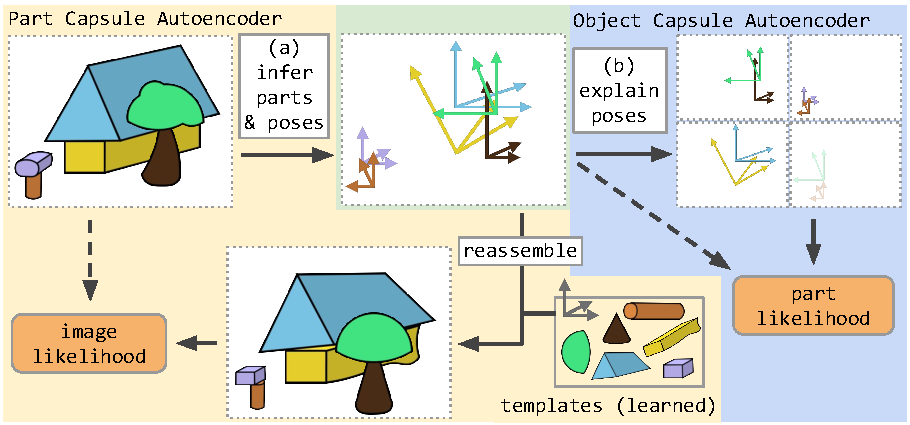
\includegraphics[width=.68\linewidth]{figures/SCA/blocks_v4}
        % \vspace*{-1.5em}
%    \end{minipage}
%    \hfill
%    \begin{minipage}[c]{0.3\linewidth}
%        \centering
        \caption{
            Stacked Capsule Autoencoder (\textsc{scae}):
            % \arcfull{}{SCA}
            (a) \textit{part} capsules segment the input into parts and their poses. The poses are then used to reconstruct the input by affine-transforming learned templates.
            (b) \textit{object} capsules try to arrange inferred poses into objects, thereby discovering underlying structure.
            \textsc{scae} is trained by maximizing image and part log-likelihoods subject to sparsity constraints.
        }
        \label{fig:capsule_arch}
        % \vspace*{-1.5em}
%    \end{minipage}
%    \vspace*{-.75em}
\end{figure}

% \Gls{SCA} has two stages (\cref{fig:capsule_arch}).
% Its first (\!\ie bottom) stage, \gls{ICAE}, segments an image into constituent parts, infers their poses, and reconstructs the image as a mixture of transformed parts.
% The second (top) stage, \gls{CAE}, tries to organize discovered parts and their poses into objects, where part poses \apart{} are derived from mixtures of predictions made by objects \awhole{}.
% Since each part is explained by a separate mixture, we do not need to route predictions between mixtures.
% This justifies dispensing with iterative procedures during inference, which can now be amortized using an arbitrary feed-forward encoder.
% The encoder's ability to deal with different viewpoints is not built-in; instead it is learned by doing inference for the affine-aware decoder.
% As \gls{SCA} is unsupervised, it can leverage potentially unlimited amounts of unlabelled data.
% % \yw{maybe say that the model is an autoencoder, where the decoder is structured with the assumptions about the geometries of objects as before? also maybe give some intuition about the decoder structuring the encoder to learn the structure we want it to learn (not sure if that makes sense)?}


\section{Stacked Capsule Autoencoders (\textsc{SCAE})}
\label{sec:caps_decoders}
Segmenting an image into parts is non-trivial, so we begin by abstracting away pixels and the part-discovery stage, and develop the \gls{CCAu} (\Cref{sec:constellation}).
It uses two-dimensional points as parts, and their coordinates are given as the input to the system. \Gls{CCAu} learns to model sets of points as arrangements of familiar constellations, each of which has been transformed by an independent similarity transform. The \gls{CCAu} learns to assign individual points to their respective constellations—without knowing the number of constellations or their individual shapes in advance.  Next, in Section 2.2, we develop the \glsreset{PCAu}\gls{PCAu} which learns to infer parts and their poses from images. Finally, we stack the \glsreset{OCAu}\gls{OCAu}, which closely resembles the \gls{CCAu}, on top of the \gls{PCAu} to form the \glsreset{SCAu}\gls{SCAu}.



\subsection{Constellation Autoencoder (\textsc{CCAE})}
\label{sec:constellation}

Let $\set{\bx_m\mid m=1,\dots,M}$ be a set of two-dimensional input points, where every point belongs to a constellation as in \Cref{fig:constellations}.
We first encode all input points (which take the role of part capsules) with Set Transformer \citep{Lee2019set}---a permutation-invariant encoder $h^\mathrm{caps}$ based on attention mechanisms---into $K$ object capsules.
An object capsule $k$ consists of a capsule feature vector $\bc_k$, its presence probability $a_k \in \interval{0, 1}$ and a $3 \times 3$ \glsreset{OV}\gls{OV} matrix, which represents the affine transformation between the object (constellation) and the viewer.
Note that each object capsule can represent only one object at a time.
Every object capsule uses a separate \gls{MLP} $\operatorname{h_k^\mathrm{part}}$ to predict $N \leq M$ part candidates from the capsule feature vector $\bc_k$.
Each candidate consists of the conditional probability $a_{k,n} \in \interval{0, 1}$ that a given candidate part exists, an associated scalar standard deviation $\lambda_{k,n}$, and a $3 \times 3$ \glsreset{OP}\gls{OP} matrix, which represents the affine transformation between the object capsule and the candidate part\footnote{Deriving these matrices from the capsule feature vector allows for deformable objects. We model \gls{OP}s as the sum of an input-dependent component and a constant bias. We encourage different capsules to specialize to different constellations by putting a strong $L_2$ penalty on the former.}.
Candidate predictions $\mu_{k,n}$ are given by the product of the object capsule \gls{OV} and the candidate \gls{OP} matrices.
We then model each input part as a Gaussian mixture, where $\mu_{k,n}$ and $\lambda_{k,n}$ are the centers and standard deviations of the isotropic components.
See \Cref{fig:capsule_arch,fig:sca_arch} for illustration; formal description follows:
\begin{align}
    &\textsc{ov}_{1:K}, \bc_{1:K}, a_{1:K} = \operatorname{h^\mathrm{caps}} (\bx_{1:M}) &\text{encode object capsule parameters,}\\
    % 
    &\textsc{op}_{k,1:N}, a_{k, 1:N}, \lambda_{k, 1:N} = \operatorname{h_k^\mathrm{part}} (\bc_k) &\text{decode candidate parameters from $c_k$'s,}\\
    % 
    &V_{k,n} = \textsc{ov}_k \textsc{op}_{k,n} &\text{decode a part pose candidate,}\\
    % 
    &\p{\bx_m}{k,n} = \gauss{\bx_m \mid \mu_{k,n}, \lambda_{k,n}} &\text{turn candidates into mixture components,}\label{eq:component}
\end{align}
\begin{equation}
    \p{\bx_{1:M}} = \prod_{m=1}^M \sum_{k=1}^K \sum_{n=1}^{N}  
    \frac{a_k a_{k,n}}{\sum_i a_i \sum_j a_{i,j}}
    \,\p{\bx_m}{k,n}\,. \label{eq:constellation_likelihood}
\end{equation}
The model is trained without supervision by maximizing the likelihood of part capsules in \Cref{eq:constellation_likelihood} subject to sparsity constraints, \textit{cf}.\ \Cref{sec:losses}.
The part capsule $m$ can be assigned to the object capsule $k^\star$ as $k^\star = \operatorname{arg\,max}_{k}~a_k a_{k,n}\;\p{\bx_m}{k,n}$.\footnote{We treat parts as independent and evaluate their probability under the same mixture model. While there are no clear 1:1 connections between parts and predictions, it seems to work well in practice.}
%\begin{figure} 
%    \centering
%    \begin{minipage}[c]{0.35\linewidth}
%        \centering
%        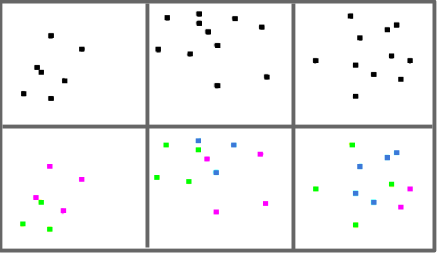
\includegraphics[width=\linewidth]{figures/SCA/consinvert5}
%    \end{minipage}
%    \hfill
%    \begin{minipage}[c]{0.63\linewidth}
%        \centering
%        \caption{
%            Unsupervised segmentation of points belonging to up to three constellations of squares and triangles at different positions, scales and orientations. 
%            The model is trained to reconstruct the points (top row) under the \gls{CCAu} mixture model. The bottom row colors the points based on the parent with highest posterior probability in the mixture model. 
%            The right-most column shows a failure case.
%            Note that the model uses sets of points, not pixels, as its input; we use images  only to visualize the constellation arrangements.
%        }
%        \label{fig:constellations}
%    \end{minipage}
%\end{figure}
\begin{SCfigure}[50]
	\centering
%	\begin{minipage}[c]{0.35\linewidth}
%		\centering
		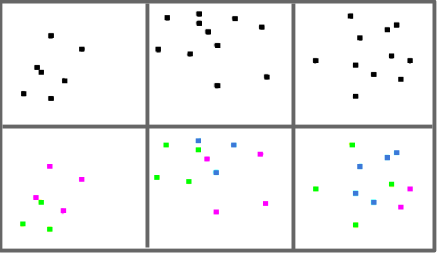
\includegraphics[width=.35\linewidth]{figures/SCA/consinvert5}
%	\end{minipage}
%	\hfill
%	\begin{minipage}[c]{0.63\linewidth}
%		\centering
		\caption{
			Unsupervised segmentation of points belonging to up to three constellations of squares and triangles at different positions, scales and orientations. 
			The model is trained to reconstruct the points (top row) under the \gls{CCAu} mixture model. The bottom row colors the points based on the parent with highest posterior probability in the mixture model. 
			The right-most column shows a failure case.
			Note that the model uses sets of points, not pixels, as its input; we use images  only to visualize the constellation arrangements.
		}
		\label{fig:constellations}
%	\end{minipage}
\end{SCfigure}
Empirical results show that this model is able to perform unsupervised instance-level segmentation of points belonging to different constellations, even in data which is difficult to interpret for humans. See \Cref{fig:constellations} for an example and \Cref{sec:constellation_expr} for details.

\subsection{Part Capsule Autoencoder (\textsc{PCAE})}
\label{sec:img_capsule}
Explaining images as geometrical arrangements of parts requires first inferring what parts the images are composed of, as well as the relationships of the parts to the viewer (which we call their poses). For the \gls{CCAu} a part is just a 2D point, but here each part capsule has a six \gls{DOF} pose, a presence variable and a unique identity. We frame the part-discovery problem as auto-encoding: the encoder learns to infer the poses and presences of different part capsules, while the decoder learns an image template for each part (\cref{fig:learned_templates}) similar to \cite{Tieleman2014thesis,Eslami2016air}. The templates corresponding to present parts are affine-transformed using their poses, and the pixels of these transformed templates are used to create a separate mixture model for each image pixel.
The \gls{PCAu} is followed by an \glsreset{OCAu}\gls{OCAu}, which closely resambles the \gls{CCAu} and is described in \Cref{sec:ocae}.

Let $\by \in \interval{0, 1}^{h \times w \times c}$ be the image.
We limit the maximum number of part capsules to $M$ and use an encoder to infer their poses $\bx_m \in \RR^6$, presence probabilities $d_m \in \interval{0, 1}$, and special features $\bz_m \in \RR^{c_z}$, one per part capsule.
The latter do not take part in direct image reconstruction, but inform the \gls{OCAu} about special aspects of the corresponding part; they are trained by backpropagating derivatives from the \gls{OCAu}.

At present, we do not allow multiple occurrences of the same type of part in an image, so the part capsules themselves are not replicated across space, though they could be.
However, we do need to recognize the part wherever it occurs in the image, and therefore the encoder consists of a \gls{CNN} with a bottom-up attention mechanism; for every part capsule $k$, it predicts a feature map $\bf{e}_k$ of $6 \text{\,(pose)} + 1 \text{\,(presence)} + c_z \text{\,(special features)}$ capsule parameters with spatial dimensions $h_e \times w_e$\,, as well as a single-channel attention mask $\bf{a}_k$.
The final parameters for that capsule are computed as $\sum_{i} \sum_j \bf{e}_{k, i,j} \operatorname{softmax}(\bf{a})_{k,i,j}$, where $\operatorname{softmax}$ is along the spatial dimensions.
This is similar to global average pooling, but allows some spatial locations to contribute to the final result more than others; we call this approach \textit{attention-based pooling}. Its effect on the model performance is analyzed in \Cref{sec:ablation}.

The image pixels are modelled as independent Gaussian mixtures.
For every pixel, we take the corresponding pixels of the transformed templates and treat them as centers of isotropic Gaussian components with constant variance.
Their mixing probabilities are proportional to both presence probabilities of part capsules and a function $f_c: \RR^c \mapsto \interval{0, 1}$ of the color value at that location\footnote{
Templates are assumed to be sparse; if there exists a template that has a non-zero value at a given location, then this templates should be used.}, where $c$ is the number of image channels. 
More formally:
\begin{align}
    &\bx_{1:M}, d_{1:M}, \bz_{1:M} = \operatorname{h^{\mathrm{enc}}}(\by) \qquad\text{encode the image to part capsule params,}\\
    &\widehat{T}_m = \operatorname{TransformImage} (T_m, \bx_m)  \qquad\text{affine transforms image templates,}\\
    % 
    &p^y_{m,i,j} \propto d_m \operatorname{f_c}\left(\widehat{T}_{m,i,j}\right) \qquad\text{compute mixing probabilities,}\\
    % 
    &\p{\by} = \prod_{i,j} \sum_{m=1}^M p^y_{m,i,j}\, \gauss{y_{i,j} \mid \widehat{T}_{m,i,j}, \sigma^2_y} \qquad\text{calculate image likelihood.} \label{eq:im_likelihood}
\end{align}

\subsection{Object Capsule Autoencoder (\textsc{OCAE})}
\label{sec:ocae}
% \todo{\ak{explain why constellation and object aes are differnet}}

The next step is to find objects in the already discovered parts\footnote{
    Discovered objects are {\it not} used top-down to refine the presences or poses of the parts during inference. However, the derivatives backpropagated via \gls{OCAu} refine the lower-level encoder network that infers the parts.
}.
To do so, we use concatenated poses $\bx_m$, special features $\bz_m$ and flattened templates $T_m$ (which convey the identity of the part capsule)
as an input to the \gls{OCAu}, which differs from the \gls{CCAu} in the following ways.
Firstly, we feed part capsule presence probabilities $d_m$ into the \gls{OCAu}'s encoder---these are used to bias the Set Transformer's attention mechanism to not take absent points into account.
% ; see \Cref{app:set_transformer} for details.
Secondly, $d_m$'s are also used to weigh the part-capsules' log-likelihood, \textit{cf}. \Cref{eq:constellation_likelihood}.
Additionally, we stop the gradient on all of \gls{OCAu}'s inputs except the special features to improve training stability and avoid the problem of collapsing latent variables; see\eg \cite{Rasmus2015ladder}.
Finally, parts discovered by the \gls{PCAu} have independent identities (templates and special features rather than 2D points).
Therefore, every part-pose is explained as an independent mixture of predictions from object-capsules---where every object capsule makes exactly $M$ candidate predictions $V_{k,1:M}$, or exactly {\bf one} candidate prediction per part.
Consequently, the part-capsule likelihood is given by,
\begin{equation}
    \p{\bx_{1:M}, d_{1:M}} = \prod_{m=1}^M \left[\, \sum_{k=1}^K  
    \frac{a_k a_{k,m}}{\sum_i a_i \sum_j a_{i,j}}
    \,\p{\bx_m}{k,m}\right]^{d_m}\,. \label{eq:mod_constellation_likelihood}
\end{equation}

%\begin{figure}
%    \centering
%    \begin{minipage}[b]{.47\linewidth}
%    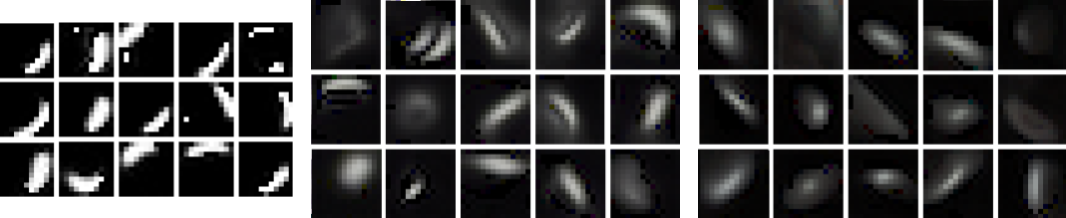
\includegraphics[width=\linewidth]{figures/SCA/templates}
%    \end{minipage}
%    \hfill
%    \begin{minipage}[b]{.52\linewidth}
%    \caption{Templates learned on \textsc{mnist} (left) as well as sobel-filtered \textsc{svhn} (middle) and \textsc{cifar10} (right). In each case templates converge to strokes. For \textsc{svhn} they often take the form of double strokes---this is due to sobel filtering, which effectively extracts edges.}
%    \label{fig:learned_templates}
%    \end{minipage}
%\end{figure}
\begin{figure}
	\centering
		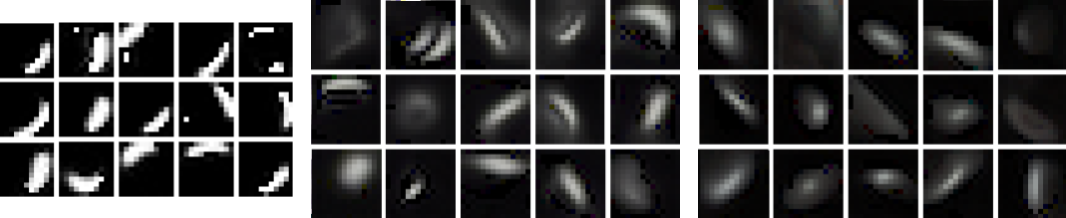
\includegraphics[width=.85\linewidth]{figures/SCA/templates}
		\caption{Templates learned on \textsc{mnist} (left) as well as sobel-filtered \textsc{svhn} (middle) and \textsc{cifar10} (right). In each case templates converge to strokes. For \textsc{svhn} they often take the form of double strokes---this is due to sobel filtering, which effectively extracts edges.}
		\label{fig:learned_templates}
\end{figure}
\begin{figure}
    \centering
    \begin{subfigure}[c]{.09\linewidth}
        
\includegraphics[width=\linewidth]{figures/SCA/mnist/inputs}
        \caption{}
    \end{subfigure}
    \hfill
    \begin{subfigure}[c]{.09\linewidth}
        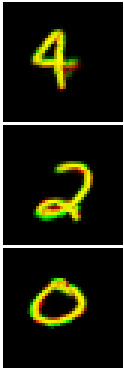
\includegraphics[width=\linewidth]{figures/SCA/mnist/recs}
        \caption{}
    \end{subfigure}
        \hfill
    \begin{subfigure}[c]{.059\linewidth}
        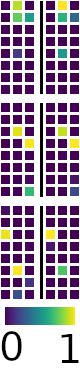
\includegraphics[width=\linewidth]{figures/SCA/mnist/acts}
        \caption{}
    \end{subfigure}
    \hfill
    \begin{subfigure}[c]{.18\linewidth}
        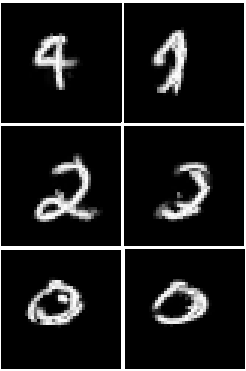
\includegraphics[width=\linewidth]{figures/SCA/mnist/caps_recs}
        \caption{}
    \end{subfigure}
    \hfill
    \begin{subfigure}[c]{.45\linewidth}
        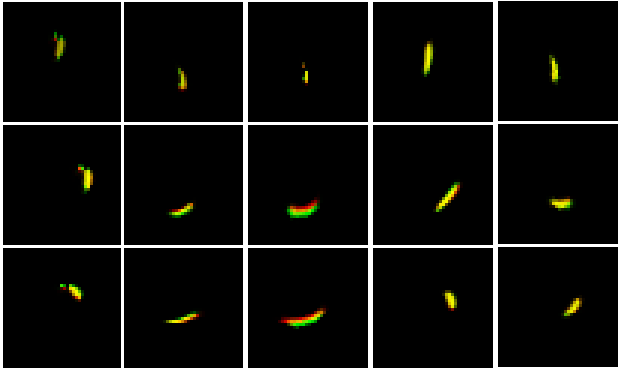
\includegraphics[width=\linewidth]{figures/SCA/mnist/transformed_templates}
        \caption{}
    \end{subfigure}
%    \hfill
%    \begin{minipage}[c]{.52\linewidth}
        \caption{
        $40\times40$ \textsc{mnist} (a) images and their (b) reconstructions from part capsules in red and object capsules in green, with overlapping regions in yellow.
        Only a few object capsules are activated for every input (c) a priori (left) and even fewer are needed to reconstruct it (right).
        The most active capsules (d) capture object identity and the majority of information about its appearance. 
        Finally, (e) affine-transformed templates show how exactly parts are used to reconstruct the images.
        }
        \label{fig:mnist_rec}
%    \end{minipage}
\end{figure}
\subsection{Achieving Sparse and Diverse Capsule Presences}
\label{sec:losses}
Stacked Capsule Autoencoders are trained to maximise pixel and part log-likelihoods ($\loss[\mathrm{ll}]{} = \log\p{\by} + \log\p{\bx_{1:M}}$).
If not constrained, however, they tend to either use all of the part and object capsules to explain every data example, or collapse onto using always the same subset of capsules, regardless of the input.
We would like the model to use different sets of part-capsules for different input examples and to specialize object-capsules to particular arrangements of parts; to encourage this, we impose sparsity and entropy constraints.  We evaluate their importance in \Cref{sec:ablation}.

We first define prior and posterior object-capsule presence as follows.
For a minibatch of size {\small$B$} with {\small$K$} object capsules and $M$ part capsules we define a minibatch of prior capsule presence $a^\mathrm{prior}_{1:K}$ with dimension {\small$[B, K]$} and posterior capsule presence $a^\mathrm{posterior}_{1:K,1:M}$ with dimension {\small$[B, K, M]$} as,
\begin{equation}
    a^\mathrm{prior}_k = a_k \max_m a_{m,k}\,,
    \qquad
    a^\mathrm{posterior}_{k,m} = a_k a_{k,m}\;\gauss{\bx_m \mid m,k}\,,
\end{equation}
respectively; the former is the maximum presence probability among predictions from object capsule $k$ while the latter is the unnormalized mixing probability used to explain part capsule~$m$.
\begin{description}[leftmargin=\parindent]
\item[Prior sparsity]
    Let $\overline{u}_k = \frac{1}{B} \sum_{b=1}^B a^\mathrm{prior}_{b,k}$ the average presence probability of the object capsule $k$ among different training examples, and $\widehat{u}_b = \sum_{k=1}^K a^\mathrm{prior}_{b,k}$ the sum of object capsule presence probabilities for a given example.
    If we assume that training examples contain objects from different classes uniformly at random and we would like to assign the same number of object capsules to every class then each class would obtain $\nicefrac{K}{C}$ capsules.
    Moreover, if we assume that only one object is present in every image, then $\nicefrac{B}{C}$ object capsules should be present for every input example.
    To this end, we minimize,
    \begin{equation}
        \loss[\mathrm{prior}]{} = 
        \frac{1}{B} \sum_{b=1}^B ||\widehat{u}_b  - \frac{K}{C} ||_2
        +
         \frac{1}{K} \sum_{k=1}^K || \overline{u}_k  - \frac{B}{C} ||_2\,. \label{eq:prior_sparsity}
    \end{equation}
    % 
\item[Posterior Sparsity]
    Similarity, let $\overline{v}_k$ and $\widehat{v}_b$ be the the normalized versions of  $\sum_{k,m} a^\mathrm{posterior}_{b,k,m}$
    and $\sum_{b,m} a^\mathrm{posterior}_{b,k,m}$, respectively.
    We find it beneficial to minimize the within-example entropy of capsule posterior presence $\mathcal{H}(\overline{v}_k)$ and maximize its between-example entropy $\mathcal{H}(\widehat{v}_b)$, where $\mathcal{H}$ is the entropy \todo{\ak{say why it is beneficial}}. The final loss reads as,
    \begin{equation}
        \loss[\mathrm{posterior}]{} = \frac{1}{K} \sum_{k=1}^K \mathcal{H}(\overline{v}_k) - \frac{1}{B} \sum_{b=1}^B \mathcal{H}(\widehat{v}_b)\,. \label{eq:posterior_sparsity}
    \end{equation}
% 
\item[Every active object capsule should explain at least two parts]
    We say that an object capsule has `won' a part if it has the highest posterior mixing probability for that part among other object capsules.
    We then create binary labels for each of object capsules, where the label is $1$ if the capsule wins at least two parts and it is $0$ otherwise.
    The final loss takes the form of binary cross-entropy between the generated label and the prior capsule presence. This loss is used only for the stand-alone constellation model experiments on point data, \textit{cf}. \Cref{sec:constellation,sec:constellation_expr}.
% 
\end{description}
\begin{figure}
    \centering
    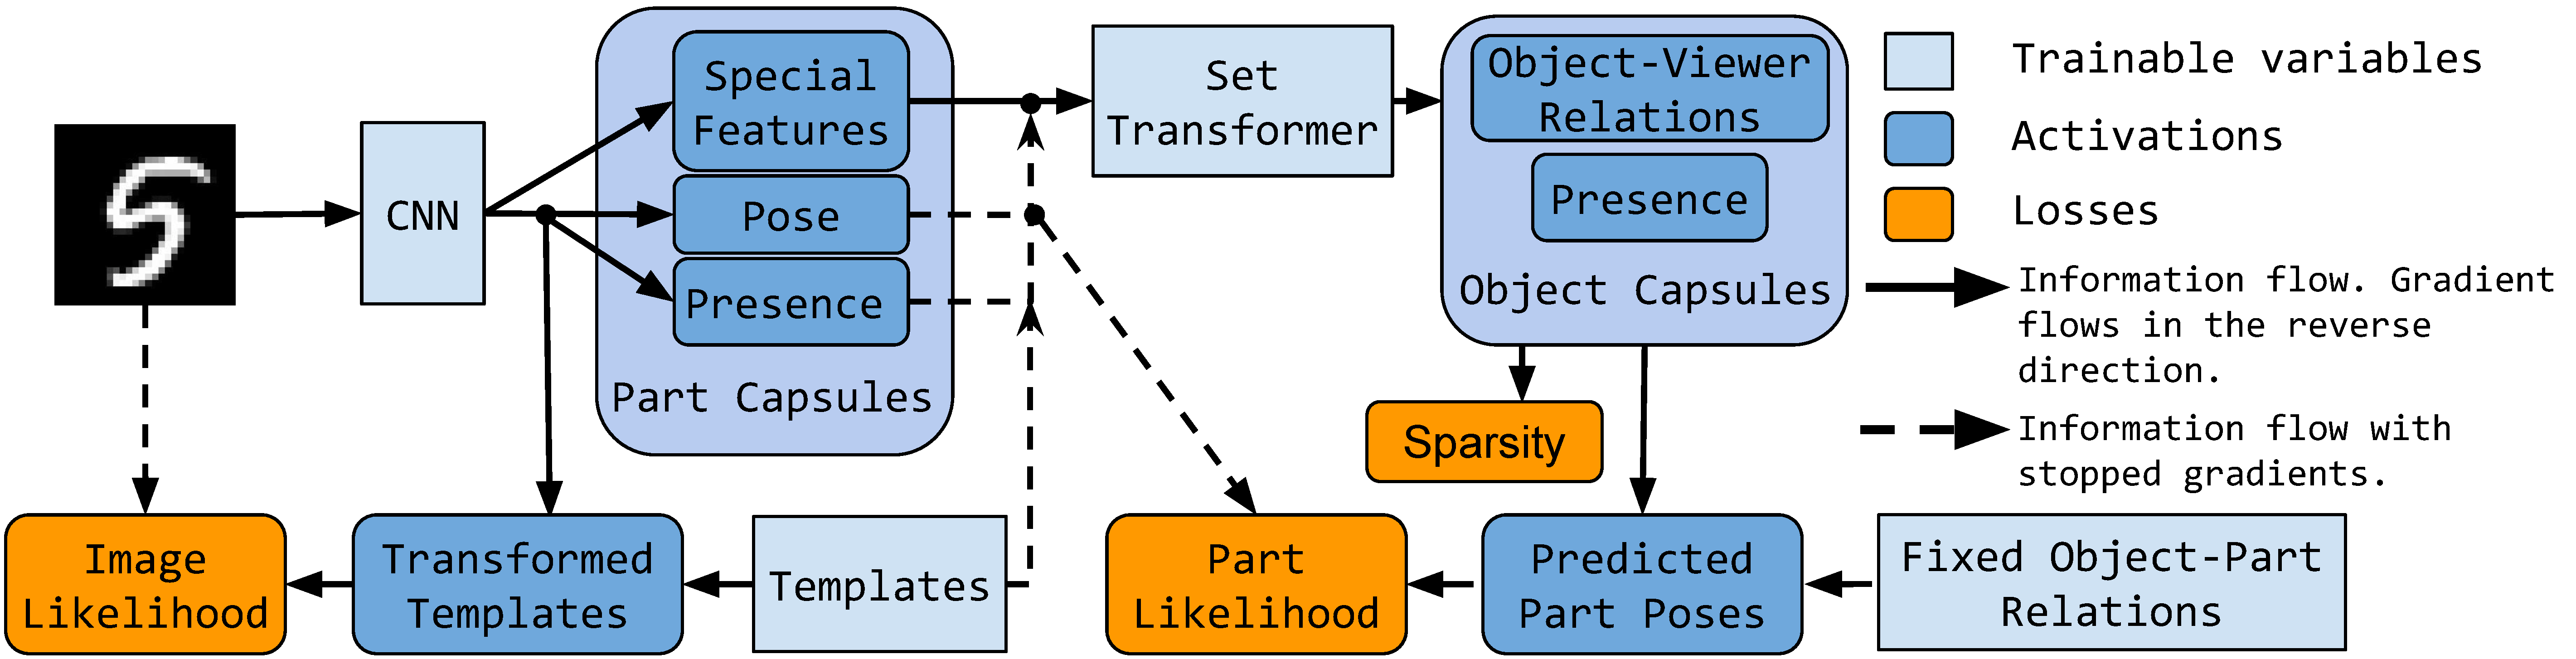
\includegraphics[width=\linewidth]{figures/SCA/sca_architecture_v3}
    \caption{\gls{SCAu} architecture.}
    \label{fig:sca_arch}
\end{figure}
\cref{fig:sca_arch} shows the schematic architecture of \gls{SCAu}. We optimize a weighted sum of image and part likelihoods and the auxiliary losses. 
Loss weight selection process as well as the values used for experiments are explained in \Cref{app:models}.

In order to make the values of presence probabilities ($a_k, a_{k,m}$ and $d_m$) closer to binary we inject uniform noise $\in \interval{-2, 2}$ into logits, similar to \cite{Tieleman2014thesis}.
This forces the model to predict logits that are far from zero to avoid stochasticity and makes the predicted presence probabilities close to binary.
Interestingly, it tends to work better in our case than using the Concrete distribution \citep{Maddison2017concrete}.
\section{Evaluation}
\label{sec:sca_experiments}

% \todo{\ak{}{this is where I left yesterday}}
The decoders in the \gls{SCAu} use explicitly parameterised affine transformations
that allow the encoders' inputs to be explained with a small set of transformed objects or parts. 
The following evaluations show how the embedded geometrical knowledge helps to discover patterns in data.
% Firstly, we perform instance-level segmentation on arrangements of simple constellations of two-dimensional points.
Firstly, we show that the \gls{CCAu} discovers underlying structures in arrangements of constellations made of two-dimensional points, thereby performing instance-level segmentation.
Secondly, we pair an \gls{OCAu} with a \gls{PCAu} and investigate whether the resulting \gls{SCAu} can discover structure in real images.
Finally, we present an ablation study that shows which components of the model contribute to the results.

\subsection{Discovering Constellations}
\label{sec:constellation_expr}
% Dataset:
We create arrangements of constellations online, where every input example consists of up to 11 two-dimensional points belonging to up to three different constellations (two squares and a triangle) as well as binary variables indicating presence of the points (points can be missing).
Each constellation is included with probability $0.5$ and undergoes a similarity transformation, whereby it is randomly scaled, rotated by up to 180\textdegree\ and shifted.
Finally, every input example is normalized such that all points lie within $\interval{-1, 1}^2$.
Note that we use sets of points, and not images, as inputs to our model.

% Baseline:
We compare the \gls{CCAu} against a baseline that uses the same encoder but a simpler decoder: the decoder uses the capsule parameter vector $\bc_k$ to directly predict the location, precision and presence probability of each of the four points as well as the presence probability of the whole corresponding constellation. 
Implementation details are listed in 
\Cref{app:constellation_model}.

% Results:
Both models are trained unsupervised by maximizing the part log-likelihood.
We evaluate them by trying to assign each input point to one of the object capsules.
To do so, we assign every input point to the object capsule with the highest posterior probability for this point, \textit{cf}. \Cref{sec:constellation}, and compute segmentation accuracy (\!\ie the true-positive rate).

The \gls{CCAu} consistently achieves below $4\%$ error with the best model achieving $2.8\%$, while the best baseline achieved $26\%$ error using the same budget for hyperparameter search.
This shows that wiring in an inductive bias towards modelling geometric relationships can help to bring down the error by an order of magnitude—at least in a toy setup where each set of points is composed of familiar constellations that have been independently transformed.

\subsection{Unsupervised Class Discovery}
\label{sec:cls_experiments}

\begin{table}
\centering
    \caption{
        Unsupervised classification results in \% with (standard deviation) are averaged over 5 runs. Methods based on mutual information are shaded. Results marked with $\mathcal{y}$ use data augmentation, ${\mathcal{r}}$ use \textsc{imagenet}-pretrained features instead of images, while ${\mathcal{x}}$ are taken from \cite{Ji2018iic}. We highlight the best results and those that are are within its 98\% confidence interval according to a two-sided t test.
    }
    \label{tab:results}
    {\small
    \begin{tabular}{@{}llll@{}}
        Method & \textsc{mnist} & \textsc{cifar10} & \textsc{svhn} \\
        \midrule
        \textsc{kmeans} (\cite{Haeusser2018adc}) & 53.49 & 20.8 & 12.5 \\
        \textsc{Ae} (\cite{Bengio2007greedy})$^{\mathcal{x}}$ & 81.2 & 31.4 & - \\
        \textsc{Gan} (\cite{Radford2016gan})$^{\mathcal{x}}$ & 82.8 & 31.5 & - \\
        \rowcolor[HTML]{EFEFEF} 
        \textsc{Imsat} (\cite{Hu2017imsat})$^{\mathcal{y}, \mathcal{r}}$ & \textbf{98.4} (0.4) & 45.6 (0.8) & \textbf{57.3} (3.9) \\ 
        \rowcolor[HTML]{EFEFEF} 
        \textsc{Iic} \citep{Ji2018iic}$^{\mathcal{x}, \mathcal{y}}$ & \textbf{98.4} (0.6) & \textbf{57.6} (5.0) & - \\
        \rowcolor[HTML]{EFEFEF} 
        \textsc{Adc} \citep{Haeusser2018adc}$^\mathcal{y}$ & \textbf{98.7} (0.6) & 29.3 (1.5) & 38.6 (4.1) \\
        \midrule
        \textsc{max-act} (\gls{SCAu}) & \textbf{98.0 (.15)}  & 19.79 (1.0) & 49.07 (1.7) \\ 
        \textsc{clust-nn} (\gls{SCAu}) & \textbf{98.5 (.11)} & 19.39 (1.5) & \textbf{53.0 (3.8)}\\ 
        \textsc{lin-match} (\gls{SCAu}) & \textbf{98.5 (.10)} & 25.01 (1.0) & \textbf{55.33 (3.4)} \\ 
        \textsc{lin-pred} (\gls{SCAu}) & \textbf{98.9 (.07)} & 33.48 (0.3) & \textbf{67.27 (4.5)} \\
    \end{tabular}
	}
\end{table}
% The goal of capsule networks was always to discover objects as an arrangement of parts. If this is the case, then presence probabilities of object capsules should be highly informative of object class.
To allow for multimodality in the appearance of objects of a specific class, we typically use more object capsules than the number of class labels. We expect that the vector of presence probabilities of object capsules should be highly informative of the class label.
To test this hypothesis, we train \gls{SCAu} on \textsc{mnist}, \textsc{svhn} and \textsc{cifar10} and try to assign class labels to vectors of object capsule presences. This is done with one of the following methods: \textsc{max-act}: we search for a training example that maximally activates given object capsule and assign the corresponding label to this capsule; \textsc{cluster-nn}: we perform \textsc{kmeans} clustering into $C$ clusters and then find the training example that is the closest to each cluster’s centroid to assign a label to the cluster; \textsc{lin-match}: after finding 10 clusters\footnote{All considered datasets have 10 classes.} with \textsc{kmeans} we use bipartite graph matching \citep{Kuhn1955hungarian} to find the permutation of cluster indices that minimizes the classification error---this is standard practice in unsupervised classification, see\eg \cite{Ji2018iic};
\textsc{lin-pred}: we train a linear classifier with supervision given the presence vectors; this learns $K \times 10$ weights and $10$ biases, where $K$ is the number of object capsules, but it does not modify any parameters of the main model.

In agreement with previous work on unsupervised clustering \citep{Ji2018iic,Hu2017imsat,Hjelm2019deepinfomax,Haeusser2018adc}, we train our models and report results on full datasets (\textsc{train}, \textsc{valid} and \textsc{test} splits).
The linear transformation used in \textsc{lin-pred} variant of our method is trained on the \textsc{train} split of respective datasets while its performance on the \textsc{test} split is reported.

We used an \gls{PCAu} with 24 single-channel $11\times11$ templates for \textsc{mnist} and 24 and 32 three-channel $14\times14$ templates for \textsc{svhn} and \textsc{cifar10}, respectively.
We used sobel-filtered images as the reconstruction target for \textsc{svhn} and \textsc{cifar10}, as in \cite{Jaiswal2018capsule}, while using the raw pixel intensities as the input to \gls{PCAu}.
The \gls{OCAu} used 24, 32 and 64 object capsules, respectively.
Further details on model architectures and hyper-parameter tuning are available in \Cref{app:models}.
All results are presented in \Cref{tab:results}.
\gls{SCAu} achieves competitive results in unsupervised object classification on \textsc{mnist} and \textsc{svhn} and under-performs slightly on \textsc{cifar10}, which is further discussed in \Cref{sec:sca_discussion}.

\subsection{Ablation study}
\label{sec:ablation}
\gls{SCAu}s have many moving parts;
an ablation study shows which model components are important and to what degree.
We train \gls{SCAu} variants on \textsc{mnist} as well as a padded-and-translated $40\times40$ version of the dataset, where the original digits are translated up to 6 pixels in each direction.
Trained models are tested on \textsc{test} splits of both datasets; additionally, we evaluate the model trained on the $40\times40$ \textsc{mnist} on the \textsc{test} split of \textsc{affnist} dataset.
Testing on \textsc{affnist} shows whether the model can generalize to unseen viewpoints.
This task was used by \cite{Rawlinson2018sparsecaps} to evaluate Sparse Unsupervised Capsules, which achieved $90.12\%$ accuracy. \Gls{SCAu} achieves $92.2\pm 0.59\%$, which indicates that it is better at viewpoint generalization.
We choose the \textsc{lin-match} performance metric, since it is the one favoured by the unsupervised classification community.
\begin{table}
\centering
    \caption{
        Ablation study on \textsc{mnist}. All used model components contribute to its final performance. \textsc{Affnist} results show out-of-distribution generalization properties and come from a model trained on $40\times40$ \textsc{mnist}. Numbers represent average \% and (standard deviation) over 10 runs. We highlight the best results and those that are are within its 98\% confidence interval according to a two-sided t test.
    }
    \label{tab:ablation}
    {\small
    \begin{tabular}{@{}lllll@{}}
        & Method & \textsc{mnist} & $40\times40$ \textsc{mnist} & \textsc{affnist} \\
        \midrule
        &full model & \textbf{97.0 (.87)} & \textbf{98.5 (.1)} & \textbf{92.2 (.59)} \\
        \midrule
        & no posterior sparsity  & \textbf{96.7	(.7)} & \textbf{98.2	(.48)} & 87.6	(1.63) \\
        a)& no prior sparsity  & 90.5 (7.56) & 94.0	(3.03) & 74.0	(4.94) \\
        & no prior/posterior sparsity  &	63.0	(13.48) &	62.7	(10.46) & 40.7 (6.81)\\
        \midrule
        & no noise in object caps &	\textbf{96.4	(1.41)} &	\textbf{97.8	(.67)} &	\textbf{90.8	(2.97)}\\
        b)& no noise in any caps &	84.8	(6.22) &	85.1	(13.13) &	76.3	(12.89)\\
        &no noise in part caps	& 83.9	(7.57) &	80.2	(9.1) &	73	(9.04)\\
        \midrule
        c)& similarity transforms &	90.4	(13.78) &	\textbf{97.4	(.99)} &	\textbf{90.1	(2.62)}\\
        &no deformations	& 87.6	(6.13) &	95.2	(1.04) &	87.6	(1.26)\\
        \midrule
        d)&\textsc{linear} part enc & \textbf{94.8	(3.0)} &	98.1	(.26)	& 76.3	(2.22)\\
        &\textsc{conv} part enc &	\textbf{96.3	(.85)} &	\textbf{97.8	(.95)} &	80.1	(2.58)\\
        \midrule
        e)& \gls{MLP} enc for object caps	& 73.0	(6.34) &	70.3	(11.2) &	52.5	(11.29)\\
        f)& no special features &	63.1	(10.55) &	66.9	(23.59) &	50.5	(18.26)\\
    \end{tabular}
	}
\end{table}
Results are split into several groups and shown in \Cref{tab:ablation}.
We describe each group in turn.
Group a) shows that sparsity losses introduced in \Cref{sec:losses} increase model performance, but that the posterior loss might not be necessary.
Group b) checks the influence of injecting noise into logits for presence probabilities, \textit{cf}. \Cref{sec:losses}.  Injecting noise into part capsules seems critical, while noise in object capsules seems unnecessary---the latter might be due to sparsity losses.
Group c) shows that using similarity (as opposed to affine) transforms in the decoder can be restrictive in some cases, while not allowing deformations hurts performance in every case.

Group d) evaluates the type of the part-capsule encoder.
The \textsc{linear} encoder entails a \gls{CNN} followed by a fully-connected layer, while the \textsc{conv} encoder predicts one feature map for every capsule parameter, followed by global-average pooling. 
The choice of part-capsule encoder seems not to matter much for within-distribution performance; however, our attention-based pooling does achieve much higher classification accuracy when evaluated on a different dataset, showing better generalization to novel viewpoints.

Additionally, e) using Set Transformer as the object-capsule encoder is essential.
We hypothesize that it is due to the natural tendency of Set Transformer to find clusters, as reported in \cite{Lee2019set}.
Finally, f) using special features $\bz_m$ seems not less important---presumably due to effects the high-level capsules have on the representation learned by the primary encoder.
%Previous capsule networks use the poses of parts and the discriminatively learned part->object relationships to cast votes for the poses of objects and then look for clusters among these votes.



% \yw{edited for anonymity}
%Capsule networks\footnote{A \textit{capsule} is a group of neurons representing a single concept, whose output is a feature vector; the term can sometimes be used to refer to the vector, too.} \citep{Hinton2018capsule} use this insight by modelling object parts explicitly. They predict the affine transformations between object parts \apart{} and camera \acamera{} coordinate frames (parts' \textit{pose}) and learn transformations between part \apart{} and object \awhole{} coordinate frames.
% \todo{\ak{don't remove the icons! they help me understand text and I'm sure others will appreciate, too}}


%Capsules do have several drawbacks, however, related to how they predict whole objects: each part makes a separate prediction for a whole, which is assumed to be present when predictions of many parts agree.
%

% \ak{yeah, like we don't have hyperparameters...}
% (i) they are sensitive to the threshold for how tightly the predictions of the parts should agree,
%(i) capsules use iterative inference to ensure that a part is included in only one whole;
% (ii) the pose of each part needs to have the same dimensionality as the pose of the whole if it is to make a point prediction for the latter, and
%(ii) since every part \apart{} has to make a point prediction for the pose of a whole \awhole{}, both poses need to have the same dimensionality; and
%(iii) learning is supervised.
\vspace{-1pt}
\section{Related Work}
\label{sec:related_work}\vspace{-5pt}

\textbf{Capsule Networks}\ \ 
Our work combines ideas from Transforming Autoencoders \citep{Hinton2011tae} and \textsc{em} Capsules \citep{Hinton2018capsule}.
Transforming autoencoders discover affine-aware capsule \textit{instantiation parameters} by training an autoencoder to predict an affine-transformed version of the input image from the original image plus an extra input, which explicitly represents the transformation.
By contrast, our model does not need any input other than the image.

Both \textsc{em} Capsules and the preceding Dynamic Capsules \citep{Sabour2017capsule} use the poses of parts and learned part$\rightarrow$object relationships to vote for the poses of objects. When multiple parts cast very similar votes, the object is assumed to be present, which is facilitated by an interactive inference (routing) algorithm. Iterative routing is inefficient and has prompted further research. \cite{wang2018optimization} formulated routing as an optimization of a clustering loss and a \textsc{kl}-divergence-based regularization term.  \cite{zhang2018fast} proposed a weighted kernel density estimation-based routing method. \cite{encapsule} proposed approximating routing with two branches and sending feedback via optimal transport divergence between two distributions (lower and higher capsules). 
In contrast to prior work, we use objects to predicts parts rather than vice-versa, therefore we can dispense with iterative routing at inference time. The encoder of the \gls{OCAu} learns how to group parts into objects and it respects the single parent constraint, because it is trained using derivatives produced by a decoder that uses a mixture model of parts which assumes that each part must be explained by a single object. 

Additionally, since it is the objects that predict parts, the parts are allowed to have fewer degrees-of-freedom in their poses than objects (as in the \gls{CCAu}). 
Inference is still possible, because the \gls{OCAu} encoder makes object predictions based on {\it all} the parts rather than an individual part.

A further advantage of our version of capsules is that it can perform unsupervised learning. Previous versions of capsules used discriminative learning, though \cite{sparsecaps} used the reconstruction \gls{MLP} introduced in \cite{Sabour2017capsule} to train Dynamic Capsules without supervision and has shown that unsupervised training for capsule-conditioned reconstruction helps with generalization to \textsc{affnist} classification; we further improve on their results, \textit{cf}.\ \Cref{sec:ablation}.

% \comment{ by maximizing the likelihood of part poses under mixtures of predictions made by different object capsules.
% Moreover, our method is trained without supervision while the previous approaches require supervised training.}
% 
% \ak{}{the following is irrelevant to this work}
% \cite{lalonde} proposed a deconvolutional capsule network for object segmentation and \cite{duarte} introduced capsule pooling for action segmentation and classification. 
% \cite{jaiswal,upadhyay,saqur} developed Capsule\textsc{gan}s, which have shown better 2D image generation quality.

% \cite{zhao20183d} proposed Capsules as disjoint latent basis functions to summarize point clouds and learned the embedded latent capsules via dynamic routing.
% These are similar to our method, with the difference that we use an affine-aware capsule decoder to replace routing and reconstruct images.

\textbf{Unsupervised Classification}\ \ 
There are two main approaches to unsupervised object category detection in computer vision.
The first one is based on representation learning and typically requires discovering clusters or learning a classifier on top of the learned representation.
\cite{Eslami2016,Kosiorek2018sqair} use an iterative procedure to infer a variable number of latent variables, one for every object in a scene, that are highly informative of object class, while \cite{Greff2019multi,Burgess2019monet} perform unsupervised instance-level segmentation in an iterative fashion.
While similar to our work, these approaches cannot decompose objects into their constituent parts and do not provide explicit description of object shape (\!\eg templates and their poses in our model).

The second approach targets classification explicitly by minimizing mutual information (\textsc{mi})-based losses and directly learning class-assignment probabilities.
\textsc{Iic} \citep{iic} maximizes an exact estimator of \textsc{mi} between two discrete probability vectors describing (transformed) versions of the input image.
DeepInfoMax \citep{Hjelm2019deepinfomax} relies on negative samples and maximizes \textsc{mi} between the predicted probability vector and its input via noise-contrastive estimation \citep{Gutmann2010nce}.
This class of methods directly maximizes the amount of information contained in an assignment to discrete clusters and they hold state-of-the-art results on most unsupervised classification tasks.
\textsc{Mi}-based methods suffer from typical drawbacks of mutual information estimation: they require heavy data augmentation and large batch sizes.
This is in contrast to our method, which achieves comparable performance with batch size no bigger than 128 and with no data augmentation.

\textbf{Geometrical Reasoning}\ \ 
Other attempts at incorporating geometrical knowledge into neural networks include exploiting equivariance properties of group transformations \citep{Cohen2016group} or new types of convolutional filters \citep{mallat,kocvok}.
Although they achieve significant parameter efficiency in handling rotations or reflections compared to standard \glspl{CNN}, these methods cannot handle additional degrees of freedom of affine transformations---like scale. \cite{lenssen} combined capsule networks with group convolutions to  guarantee equivariance and invariance in capsule networks.
Spatial Transformers (\textsc{st}; \cite{Jaderberg2015}) apply affine transformations to the image sampling grid while steerable networks \citep{Cohen2016steerable,Jacobsen2017dynamic} dynamically change convolutional filters.
These methods are similar to ours in the sense that transformation parameters are predicted by a neural network, but differ in the sense that \textsc{st} uses global transformations applied to the whole image while steerable networks use only local transformations.
Our approach can use different global transformations for every object as well as local transformations for each of their parts.

% \ak{}{I think we can skip GQN and HoloGAN}
% Novel view synthesis is an emerging task which requires affine-aware representation learning. 
% \Gls{GQN} \citep{Eslami2016} is closely related to transforming autoencoders: it learns to represent a whole three-dimensional scene in its latent variable computed from multiple viewpoints and trains an affine-aware decoder to reconstruct the scene from a given viewpoint.
% More recently HoloGAN \citep{hologan} has been able to generate new viewpoints without any supervision. HoloGAN applies random 3D affine transformations on learned templates to disentangle pose from shape and therefore is able to generate new viewpoints of the same shape.




\section{Discussion}\vspace*{-5pt}
\label{sec:sca_discussion}
    The main contribution of our work is a novel method for representation learning, in which highly structured decoder networks are used to train one encoder network that can segment an image into parts and their poses and another encoder network that can compose the parts into coherent wholes.
    Despite the fact that our training objective is not concerned with classification or clustering,
    \gls{SCAu} is the only method that achieves competitive results in unsupervised object classification without relying on mutual information (\textsc{mi}).
    This is significant, since unlike our method, \textsc{mi}-based methods require sophisticated data augmentation.
    It may be possible to further improve results by using an \textsc{mi}-based loss to train \gls{SCAu}, where the vector of capsule probabilities could take the role of discrete probability vectors in \textsc{Ji2018iic} \citep{Iic}.
    \gls{SCAu} under-performs on \textsc{cifar10}, which could be because of using fixed templates, which are not expressive enough to model real data.
    This might be fixed by building deeper hierarchies of capsule autoencoders (\!\eg complicated scenes in computer graphics are modelled as deep trees of affine-transformed geometric primitives) as well as using input-dependent shape functions instead of fixed templates---both of which are promising directions for future work.
    It may also be possible to make a much better \gls{PCAu} for learning the primary capsules by using a differentiable renderer in the generative model that reconstructs pixels from the primary capsules.
    
    Finally, the \gls{SCAu} could be the `figure' component of a mixture model that also includes a versatile `ground' component  that can be used to account for everything except the figure.  A complex image could then be analyzed using sequential attention to perceive one figure at a time. 

\section{Acknowledgements}
We would like to thank Sandy H.\,Huang for help with editing the manuscript and making \Cref{fig:capsule_arch}.
Additionally, we would like to thank S.\,M.\,Ali Eslami and Danijar Hafner for helpful discussions throughout the project. We also thank Hyunjik Kim, Martin Engelcke, Emilien Dupont and Simon Kornblith for feedback on initial versions of the manuscript.q

\printbibliography

\newpage
% \FloatBarrier
\appendix
\section{Model Details}
\label{app:models}

\subsection{Constellation Experiments}
\label{app:constellation_model}
% Implementation:
The \gls{CCAu} uses a four-layer Set Transformer as its encoder.
Every layer has four attention heads, 128 hidden units per head, and is followed by layer norm \citep{Ba2016LayerN}.
The encoder outputs three 32-dimensional vectors---one for each object capsule.
The decoder uses a separate neural net for each object capsule to predict all parameters used to model its points: this includes four candidate part predictions per capsule for a total of 12 candidates.
In this experiment, each object$\rightarrow$part relationship \gls{OP} is just a 2-D offset in the object's frame of reference (instead of a $3\times3$ matrix) and it is affine transformed by the corresponding \gls{OV} matrix to predict the 2-D point.

\subsection{Image Experiments}

We use a convolutional encoder for part capsules and a set transformer encoder \citep{Lee2019set} for object capsules.
Decoding from object capsule to part capsules is done with \glspl{MLP}, while the input image is reconstructed with affine-transformed learned templates.
Details of the architectures we used are available in \Cref{tab:arch}.
% \comment{
\begin{center}
\centering
    \captionof{table}{
        Architecture details. \textsc{S} in the last column means that the entry is the same as for \textsc{svhn}.
    }
    \label{tab:arch}
    \small
    \begin{tabular}{@{}lllll@{}}
        Dataset & Constellation & \textsc{mnist} & \textsc{svhn} & \textsc{cifar10} \\
        \midrule
        num templates & N/A & 24 & 24 & 32\\
        template size & N/A & $11\times11$ & $14\times14$ & \textsc{s}\\
        num capsules & 3 & 24 & 32 & 64\\
        part \textsc{cnn} & N/A & 2x(128:2)-2x(128:1) & 2x(128:1)-2x(128:2) & \textsc{s} \\
        set transformer & 4x(4-128)-32  & 3x(1-16)-256 & 3x(2-64)-128 & \textsc{s}
        % \midrule
\end{tabular}
\end{center}

We use ReLu nonlinearities except for presence probabilities, for which we use sigmoids.
(128:2) for a \gls{CNN} means 128 channels with a stride of two.
All kernels are $3\times3$.
For set transformer (1-16)-256 means one attention head, 16 hidden units and 256 output units; it uses layer normalization \citep{Ba2016LayerN} as in the original paper \citep{Lee2019set} but no dropout. All experiments (apart from constellations) used 16 special features per part capsule.

For \textsc{svhn} and \textsc{cifar10}, we use normalized sobel-filtered images as the target of the reconstruction to emphasize the shape importance. \Cref{fig:svhn_recons} in \Cref{app:recs} shows examples of \textsc{svhn} and \textsc{cifar10} reconstruction.
The filtering procedure is as follows:
1) apply sobel filtering, 2) subtract the median color, 3) take the absolute value of the image, 4) normalize for image values to be $\in \interval{0, 1}$.

All models are trained with the RMSProp optimizer \citep{tieleman2012rms} $\mathrm{momentum}=.9$ and $\epsilon = \left(10 * \mathrm{batch\_size}\right)^{-2}$.
Batch size is 64 for constellations and 128 for all other datasets.
The learning rate was equal to $10^{-5}$ for \textsc{mnist} and constellation experiments (without any decay), while we run a hyperparameter search for \textsc{svhn} and \textsc{cifar10}: we searched learning rates in the range of $5*10^{-5}$ to $5*10^{-4}$ and exponential learning rate decay of 0.96 every $10^3$ or $3*10^3$ weight updates. Learning rate of $10^{-4}$ was selected for both \textsc{svhn} and \textsc{cifar10}, the decay steps was $10^3$ for \textsc{svhn} and $3*10^3$ for \textsc{cifar10}.
The $\textsc{lin-pred}$ accuracy on a validation set is used as a proxy to select the best hyperparameters---including weights on different losses, reported in \Cref{tab:hparams}.
Models were trained for up to $3*10^5$ iterations on single Tesla V100 GPUs, which took 40 minutes for constellation experiments and less than a day for \textsc{cifar10}.

\begin{center}
\centering
    \captionof{table}{
        Loss weights values. The \textit{within} and \textit{between} quantifiers in sparsity losses corresponds to different terms of \Cref{eq:prior_sparsity,eq:posterior_sparsity}.
    }
    \label{tab:hparams}
    \small
    \begin{tabular}{@{}lllll@{}}
        Dataset & Constellation & \textsc{mnist} & \textsc{svhn} & \textsc{cifar10} \\
        \midrule
        part ll weight & 1 & 1 & 2.56 & 2.075 \\
        image ll weight & N/A & 1 & 1 & 1\\
        prior within sparsity & 1  & 1 & 0.22 & 0.17 \\
        prior between sparsity & 1  & 1 & 0.1 & 0.1 \\
        posterior within sparsity & 0 & 10 & 8.62 & 1.39 \\
        posterior between sparsity & 0 & 10 & 0.26 & 7.32 \\
        too-few-active-capsules & 10 & 0 & 0 & 0
        % \midrule
\end{tabular}
\end{center}

\section{Reconstructions}
\label{app:recs}
\begin{center}
\begin{tabular}{ >{\centering\arraybackslash}m{.1\linewidth} >{\centering\arraybackslash}m{.85\linewidth}}
SVHN & 
    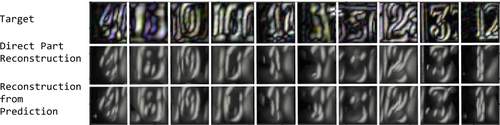
\includegraphics[width=\linewidth]{figures/SCA/svhn_recons.png}
\\
CIFAR10 & 
    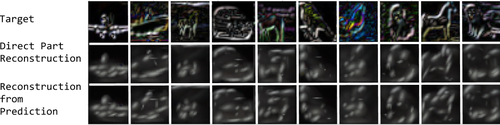
\includegraphics[width=\linewidth]{figures/SCA/cifar_recons.png}
    \end{tabular}
    \captionof{figure}{10 Sample SVHN and Cifar10 reconstructions. First row shows Sobel filtered target image. Second row shows the reconstruction from Part Capsule Layer directly. Third row shows the reconstruction if we use the object predictions for the Part poses instead of Part poses themselves for reconstruction. The templates in this model has the same number of channels as the image, but they have converged to black and white templates and the reconstruction do not have color diversity. The \gls{SCAu} model is trained completely unsupervised but the reconstructions tend to focus on the center digit in SVHN and filter the rest of the clutter. }
    \label{fig:svhn_recons}
\end{center}

% \begin{figure}
%     \centering
%     \vspace*{.5em}
%     \begin{minipage}[b]{0.58\linewidth}
%     \centering
%     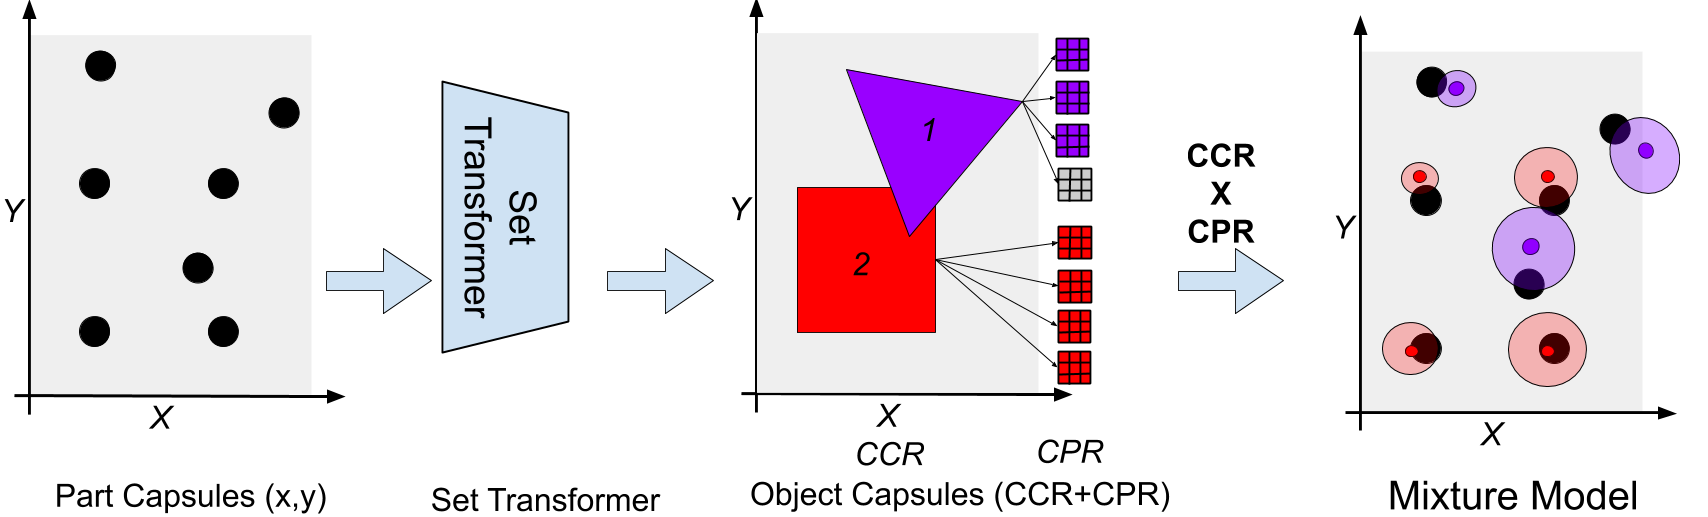
\includegraphics[width=\linewidth]{figures/SCA/constellation_read.png}
%     \vspace*{.05em}
%     \end{minipage}
%     \hfill
%     \begin{minipage}[b]{.4\linewidth}
%     \caption{Constellation Autoencoder. 
%     The set transformer encoder $h^\mathrm{caps}$ predicts parameters of two object capsules, which predict affine transformations, precisions and presences of object and part capsules. 
%     Finally, input points are explained by a mixture of predictions, where the size of the circle corresponds to its precision.
%     }
%     \label{fig:constellation_capsule}
%     \end{minipage}
% \end{figure}
% \section{Modified Set Transformer}
% \label{app:set_transformer}
% \todo{fill in}
% \printbibliography
\end{document}
